% Options for packages loaded elsewhere
\PassOptionsToPackage{unicode}{hyperref}
\PassOptionsToPackage{hyphens}{url}
%
\documentclass[
]{report}
\usepackage{amsmath,amssymb}
\usepackage{lmodern}
\usepackage{iftex}
\ifPDFTeX
  \usepackage[T1]{fontenc}
  \usepackage[utf8]{inputenc}
  \usepackage{textcomp} % provide euro and other symbols
\else % if luatex or xetex
  \usepackage{unicode-math}
  \defaultfontfeatures{Scale=MatchLowercase}
  \defaultfontfeatures[\rmfamily]{Ligatures=TeX,Scale=1}
\fi
% Use upquote if available, for straight quotes in verbatim environments
\IfFileExists{upquote.sty}{\usepackage{upquote}}{}
\IfFileExists{microtype.sty}{% use microtype if available
  \usepackage[]{microtype}
  \UseMicrotypeSet[protrusion]{basicmath} % disable protrusion for tt fonts
}{}
\makeatletter
\@ifundefined{KOMAClassName}{% if non-KOMA class
  \IfFileExists{parskip.sty}{%
    \usepackage{parskip}
  }{% else
    \setlength{\parindent}{0pt}
    \setlength{\parskip}{6pt plus 2pt minus 1pt}}
}{% if KOMA class
  \KOMAoptions{parskip=half}}
\makeatother
\usepackage{xcolor}
\usepackage{color}
\usepackage{fancyvrb}
\newcommand{\VerbBar}{|}
\newcommand{\VERB}{\Verb[commandchars=\\\{\}]}
\DefineVerbatimEnvironment{Highlighting}{Verbatim}{commandchars=\\\{\}}
% Add ',fontsize=\small' for more characters per line
\usepackage{framed}
\definecolor{shadecolor}{RGB}{248,248,248}
\newenvironment{Shaded}{\begin{snugshade}}{\end{snugshade}}
\newcommand{\AlertTok}[1]{\textcolor[rgb]{0.94,0.16,0.16}{#1}}
\newcommand{\AnnotationTok}[1]{\textcolor[rgb]{0.56,0.35,0.01}{\textbf{\textit{#1}}}}
\newcommand{\AttributeTok}[1]{\textcolor[rgb]{0.77,0.63,0.00}{#1}}
\newcommand{\BaseNTok}[1]{\textcolor[rgb]{0.00,0.00,0.81}{#1}}
\newcommand{\BuiltInTok}[1]{#1}
\newcommand{\CharTok}[1]{\textcolor[rgb]{0.31,0.60,0.02}{#1}}
\newcommand{\CommentTok}[1]{\textcolor[rgb]{0.56,0.35,0.01}{\textit{#1}}}
\newcommand{\CommentVarTok}[1]{\textcolor[rgb]{0.56,0.35,0.01}{\textbf{\textit{#1}}}}
\newcommand{\ConstantTok}[1]{\textcolor[rgb]{0.00,0.00,0.00}{#1}}
\newcommand{\ControlFlowTok}[1]{\textcolor[rgb]{0.13,0.29,0.53}{\textbf{#1}}}
\newcommand{\DataTypeTok}[1]{\textcolor[rgb]{0.13,0.29,0.53}{#1}}
\newcommand{\DecValTok}[1]{\textcolor[rgb]{0.00,0.00,0.81}{#1}}
\newcommand{\DocumentationTok}[1]{\textcolor[rgb]{0.56,0.35,0.01}{\textbf{\textit{#1}}}}
\newcommand{\ErrorTok}[1]{\textcolor[rgb]{0.64,0.00,0.00}{\textbf{#1}}}
\newcommand{\ExtensionTok}[1]{#1}
\newcommand{\FloatTok}[1]{\textcolor[rgb]{0.00,0.00,0.81}{#1}}
\newcommand{\FunctionTok}[1]{\textcolor[rgb]{0.00,0.00,0.00}{#1}}
\newcommand{\ImportTok}[1]{#1}
\newcommand{\InformationTok}[1]{\textcolor[rgb]{0.56,0.35,0.01}{\textbf{\textit{#1}}}}
\newcommand{\KeywordTok}[1]{\textcolor[rgb]{0.13,0.29,0.53}{\textbf{#1}}}
\newcommand{\NormalTok}[1]{#1}
\newcommand{\OperatorTok}[1]{\textcolor[rgb]{0.81,0.36,0.00}{\textbf{#1}}}
\newcommand{\OtherTok}[1]{\textcolor[rgb]{0.56,0.35,0.01}{#1}}
\newcommand{\PreprocessorTok}[1]{\textcolor[rgb]{0.56,0.35,0.01}{\textit{#1}}}
\newcommand{\RegionMarkerTok}[1]{#1}
\newcommand{\SpecialCharTok}[1]{\textcolor[rgb]{0.00,0.00,0.00}{#1}}
\newcommand{\SpecialStringTok}[1]{\textcolor[rgb]{0.31,0.60,0.02}{#1}}
\newcommand{\StringTok}[1]{\textcolor[rgb]{0.31,0.60,0.02}{#1}}
\newcommand{\VariableTok}[1]{\textcolor[rgb]{0.00,0.00,0.00}{#1}}
\newcommand{\VerbatimStringTok}[1]{\textcolor[rgb]{0.31,0.60,0.02}{#1}}
\newcommand{\WarningTok}[1]{\textcolor[rgb]{0.56,0.35,0.01}{\textbf{\textit{#1}}}}
\usepackage{longtable,booktabs,array}
\usepackage{calc} % for calculating minipage widths
% Correct order of tables after \paragraph or \subparagraph
\usepackage{etoolbox}
\makeatletter
\patchcmd\longtable{\par}{\if@noskipsec\mbox{}\fi\par}{}{}
\makeatother
% Allow footnotes in longtable head/foot
\IfFileExists{footnotehyper.sty}{\usepackage{footnotehyper}}{\usepackage{footnote}}
\makesavenoteenv{longtable}
\usepackage{graphicx}
\makeatletter
\def\maxwidth{\ifdim\Gin@nat@width>\linewidth\linewidth\else\Gin@nat@width\fi}
\def\maxheight{\ifdim\Gin@nat@height>\textheight\textheight\else\Gin@nat@height\fi}
\makeatother
% Scale images if necessary, so that they will not overflow the page
% margins by default, and it is still possible to overwrite the defaults
% using explicit options in \includegraphics[width, height, ...]{}
\setkeys{Gin}{width=\maxwidth,height=\maxheight,keepaspectratio}
% Set default figure placement to htbp
\makeatletter
\def\fps@figure{htbp}
\makeatother
\setlength{\emergencystretch}{3em} % prevent overfull lines
\providecommand{\tightlist}{%
  \setlength{\itemsep}{0pt}\setlength{\parskip}{0pt}}
\setcounter{secnumdepth}{5}
\newlength{\cslhangindent}
\setlength{\cslhangindent}{1.5em}
\newlength{\csllabelwidth}
\setlength{\csllabelwidth}{3em}
\newlength{\cslentryspacingunit} % times entry-spacing
\setlength{\cslentryspacingunit}{\parskip}
\newenvironment{CSLReferences}[2] % #1 hanging-ident, #2 entry spacing
 {% don't indent paragraphs
  \setlength{\parindent}{0pt}
  % turn on hanging indent if param 1 is 1
  \ifodd #1
  \let\oldpar\par
  \def\par{\hangindent=\cslhangindent\oldpar}
  \fi
  % set entry spacing
  \setlength{\parskip}{#2\cslentryspacingunit}
 }%
 {}
\usepackage{calc}
\newcommand{\CSLBlock}[1]{#1\hfill\break}
\newcommand{\CSLLeftMargin}[1]{\parbox[t]{\csllabelwidth}{#1}}
\newcommand{\CSLRightInline}[1]{\parbox[t]{\linewidth - \csllabelwidth}{#1}\break}
\newcommand{\CSLIndent}[1]{\hspace{\cslhangindent}#1}
\usepackage{booktabs}
\usepackage{geometry}
\usepackage[none]{hyphenat}
\usepackage{titlesec}
\usepackage{longtable}
\usepackage{xcolor}
\usepackage{setspace}
\usepackage{pdfpages}

\pagestyle{plain}

%%%% Set margins
\setlength{\topmargin}{-1cm}
\addtolength{\evensidemargin}{-1cm}
\addtolength{\oddsidemargin}{-1cm}
\addtolength{\textheight}{3cm}
\addtolength{\textwidth}{2cm}

% Spacing for reading guides
\newcommand{\rgs}{\vspace{12pt}} % Vertical space
\newcommand{\rgi}{\hspace{24pt}}  % Indent

\newcommand\latexcode[1]{#1}

% Format chapter titles and spacing
\renewcommand*{\chaptername}{Week}

\titleformat{\chapter}[display]
{\bfseries\Large}
{\filleft\MakeUppercase{\chaptertitlename} \Huge\thechapter}
{3ex}
{\titlerule
\vspace{1.5ex}%
\filright}
[\vspace{1.5ex}%
\titlerule]
\titlespacing*{\chapter}{0pt}{-40pt}{20pt}
\ifLuaTeX
  \usepackage{selnolig}  % disable illegal ligatures
\fi
\IfFileExists{bookmark.sty}{\usepackage{bookmark}}{\usepackage{hyperref}}
\IfFileExists{xurl.sty}{\usepackage{xurl}}{} % add URL line breaks if available
\urlstyle{same} % disable monospaced font for URLs
\hypersetup{
  hidelinks,
  pdfcreator={LaTeX via pandoc}}

\title{\textbf{STAT 216 Coursepack}\\
\strut \\

\includegraphics[width=5in,height=\textheight]{images/msu-campus.jpg}}
\usepackage{etoolbox}
\makeatletter
\providecommand{\subtitle}[1]{% add subtitle to \maketitle
  \apptocmd{\@title}{\par {\large #1 \par}}{}{}
}
\makeatother
\subtitle{Summer 2023\\
Montana State University}
\author{Melinda Yager\\
Jade Schmidt\\
Stacey Hancock}
\date{}

\begin{document}
\maketitle

\newpage
\thispagestyle{empty}

This resource was developed by Melinda Yager, Jade Schmidt, and Stacey Hancock in 2021 to accompany the online textbook: Hancock, S., Carnegie, N., Meyer, E., Schmidt, J., and Yager, M. (2021). \emph{Montana State Introductory Statistics with R}. Montana State University. \url{https://mtstateintrostats.github.io/IntroStatTextbook/}.

This resource is released under a \href{https://creativecommons.org/licenses/by-nc-sa/4.0/}{Creative Commons BY-NC-SA 4.0} license unless otherwise noted.

\setcounter{tocdepth}{1}
\addtocontents{toc}{\protect\thispagestyle{empty}}
\tableofcontents
\thispagestyle{empty}

\newpage
\setcounter{page}{1}

\hypertarget{preface}{%
\chapter*{Preface}\label{preface}}
\addcontentsline{toc}{chapter}{Preface}

This coursepack accompanies the textbook for STAT 216: Montana State Introductory Statistics with R, which can be found at \url{https://mtstateintrostats.github.io/IntroStatTextbook/}. The syllabus for the course (including the course calendar), data sets, and links to D2L Brightspace, Gradescope, and the MSU RStudio server can be found on the course webpage: \url{https://math.montana.edu/courses/s216/}.
Videos assigned in the course calendar and other notes and review materials are linked in D2L.

Each of the activities in this workbook is designed to target specific learning outcomes of the course, giving you practice with important statistical concepts in a group setting with instructor guidance. In addition to the in-class activities for the course, the coursepack includes reading guides to aid in taking notes while you complete the required readings and videos. Bring this workbook with you to class each class period, and take notes in the workbook as you would your own notes. A well-written completed workbook will provide an optimal study guide for exams!

The activities and labs in this coursepack will be completed during class time. Parts of each lab will be turned in on Gradescope. To aid in your understanding, read through the introduction for each activity before attending class each day.

STAT 216 is a 3-credit in-person course. In our experience, it takes six to nine hours per week outside of class to achieve a good grade in this class. By ``good'' we mean at least a C because a grade of D or below does not count toward fulfilling degree requirements. Many of you set your goals higher than just getting a C, and we fully support that. You need roughly nine hours per week to review past activities, read feedback on previous assignments, complete current assignments, and prepare for the next day's class. The following will give you an idea of what a typical week in the life of a STAT 216 student looks like.

\begin{itemize}
\tightlist
\item
  \emph{Prior to class meeting}:

  \begin{itemize}
  \tightlist
  \item
    Read assigned sections of the textbook, using the provided reading guides to take notes on the material.
  \item
    Watch assigned videos on that week's content, pausing to take notes and answer video quiz questions.
  \item
    Read through the introduction to the day's in-class activity.
  \item
    Read through the week's homework assignment and note any questions you may have on the content.
  \end{itemize}
\item
  \emph{During class meeting}:

  \begin{itemize}
  \tightlist
  \item
    Work through the in-class activity or weekly lab with your classmates and instructor, taking detailed notes on your answers to each question in the activity.
  \end{itemize}
\item
  \emph{After class meeting}:

  \begin{itemize}
  \tightlist
  \item
    Complete any parts of the activity you did not complete in class.
  \item
    Review the activity solutions in the Math and Stat Center, and take notes on key points.
  \item
    Finish watching any remaining assigned videos or readings for the week.
  \item
    Complete the week's homework assignment.
  \end{itemize}
\end{itemize}

\nocite{*}

\hypertarget{inference-for-two-categorical-variables-theory-based-methods}{%
\chapter{Inference for Two Categorical Variables: Theory-based Methods}\label{inference-for-two-categorical-variables-theory-based-methods}}

\hypertarget{week-9-reading-guide-theory-based-inference-for-a-difference-in-proportions}{%
\section{Week 9 Reading Guide: Theory-based Inference for a Difference in Proportions}\label{week-9-reading-guide-theory-based-inference-for-a-difference-in-proportions}}

\hypertarget{section-15.3-theory-based-inferential-methods-for-pi_1---pi_2}{%
\subsection{\texorpdfstring{Section 15.3 (Theory-based inferential methods for \(\pi_1 - \pi_2\))}{Section 15.3 (Theory-based inferential methods for \textbackslash pi\_1 - \textbackslash pi\_2)}}\label{section-15.3-theory-based-inferential-methods-for-pi_1---pi_2}}

\setstretch{1}

\textbf{Videos}

\begin{itemize}
\tightlist
\item
  15.3Tests
\item
  15.3Intervals
\end{itemize}

\setstretch{1.25}

\hypertarget{reminders-from-previous-sections}{%
\subsubsection*{Reminders from previous sections}\label{reminders-from-previous-sections}}
\addcontentsline{toc}{subsubsection}{Reminders from previous sections}

\(n\) = sample size

\(\hat{p}\) = sample proportion

\(\pi\) = population proportion

General steps of a hypothesis test:

\begin{enumerate}
\def\labelenumi{\arabic{enumi}.}
\item
  Frame the research question in terms of hypotheses.
\item
  Collect and summarize data using a test statistic.
\item
  Assume the null hypothesis is true, and simulate or mathematically model a null distribution for the test statistic.
\item
  Compare the observed test (standardized) statistic to the null distribution to calculate a p-value.
\item
  Make a conclusion based on the p-value and write the conclusion in context.
\end{enumerate}

Parameter: a value summarizing a variable(s) for a population.

Statistic: a value summarizing a variable(s) for a sample.

Sampling distribution: plot of statistics from 1000s of samples of the same size taken from the same population.

Standard deviation of a statistic: the variability of statistics from 1000s of samples; how far, on average, each statistic is from the true value of the parameter.

Standard error of a statistic: estimated standard deviation of a statistic.

Hypothesis test: a process to determine how strong the evidence of an effect is.

\rgi Also called a `significance test'.

Theory-based method: Develop a mathematical model for the sampling distribution of the statistic under the null hypothesis and use the model to calculate the probability of the observed sample statistic (or one more extreme) occurring.

Null hypothesis (\(H_0\)): the skeptical perspective; no difference; no change; no effect; random chance; what the researcher hopes to prove is \textbf{wrong}.

Alternative hypothesis (\(H_A\)): the new perspective; a difference/increase/decrease; an effect; not random chance; what the researcher hopes to prove is \textbf{correct}.

Null value: the value of the parameter when we assume the null hypothesis is true (labeled as \(parameter_0\)).

Null distribution: the simulated or modeled distribution of statistics (sampling distribution) we would expect to occur if the null hypothesis is true.

P-value: probability of seeing the observed sample data, or something more extreme, assuming the null hypothesis is true.

\(\implies\) Lower the p-value the stronger the evidence AGAINST the null hypothesis and FOR the alternative hypothesis.

Decision: a determination of whether to `reject' or `fail to reject' a null hypothesis based on a p-value and a pre-set level of significance.

Significance level (\(\alpha\)): a threshold used to determine if a p-value provides enough evidence to reject the null hypothesis or not.

\rgi Common levels of \(\alpha\) include 0.01, 0.05, and 0.10.

Statistically significant: results are considered statistically significant if the p-value is below the significance level.

Confidence interval: a process to determine how large an effect is; a range of plausible values for the parameter. Also called `estimation'.

Margin of error: the value that is added to and subtracted from the sample statistic to create a confidence interval; half the width of a confidence interval.

Confidence level: how confident we are that the confidence interval will capture the parameter.

\hypertarget{notes}{%
\subsubsection*{Notes}\label{notes}}
\addcontentsline{toc}{subsubsection}{Notes}

Conditions for the Central Limit Theorem to apply for a difference in proportions

\rgi Independence:
\rgs

\rgi \rgi Checked by:
\rgs

\rgi Success-failure condition:
\rgs

\rgi \rgi Checked by:
\rgs

\hypertarget{formulas}{%
\subsubsection*{Formulas}\label{formulas}}
\addcontentsline{toc}{subsubsection}{Formulas}

\(SD(\hat{p_1} - \hat{p_2})=\)
\rgs

Null standard error of the difference in sample proportions:
\(SE_0(\hat{p_1} - \hat{p_2})=\)
\rgs

Standardized statistic (or standardized difference in sample proportions):
\(Z=\)
\rgs

Standard error of the difference in sample proportions when we do not assume the null hypothesis is true:
\(SE(\hat{p_1} - \hat{p_2})=\)
\rgs

Theory-based confidence interval for a difference in proportions:
\rgs

Margin of error of a confidence interval for a difference in proportions:
\rgs

\hypertarget{notation}{%
\subsubsection*{Notation}\label{notation}}
\addcontentsline{toc}{subsubsection}{Notation}

Overall (pooled) proportion of successes:
\rgs

\hypertarget{example-cpr-and-blood-thinners}{%
\subsubsection*{Example: CPR and blood thinners}\label{example-cpr-and-blood-thinners}}
\addcontentsline{toc}{subsubsection}{Example: CPR and blood thinners}

\begin{enumerate}
\def\labelenumi{\arabic{enumi}.}
\item
  What are the observational units?
  \rgs
\item
  What type of study design was used? Justify your answer.
  \rgs
\item
  What is the appropriate scope of inference for these data?
  \rgs
\item
  What is the sample difference in proportions presented in this example? What notation would be used to represent this value?
  \rgs
\item
  What is the parameter (using a difference in proportions) representing in the context of this problem? What notation would be used to represent this parameter?
  \rgs
\item
  Is it valid to use theory-based methods to analyze these data?
  \rgs
  \rgs
\item
  Calculate the standard error of the difference in sample proportions without assuming a null hypothesis.
  \rgs
  \rgs
\item
  Calculate the 90\% confidence interval using \(z^*=1.65\) as the multiplier.
  \rgs
  \rgs
\end{enumerate}

\emph{Note: A confidence interval interpretation and confidence level interpretation for this example can be found in the Reading Guide solutions for Sections 15.1 and 15.2.}

\hypertarget{example-mammograms}{%
\subsubsection*{Example: Mammograms}\label{example-mammograms}}
\addcontentsline{toc}{subsubsection}{Example: Mammograms}

\begin{enumerate}
\def\labelenumi{\arabic{enumi}.}
\item
  What are the observational units?
  \rgs
\item
  What type of study design was used? Justify your answer.
  \rgs
\item
  What is the appropriate scope of inference for these data?
  \rgs
\item
  What is the sample difference in proportions presented in this example? What notation would be used to represent this value?
  \rgs
\item
  What is the parameter (using a difference in proportions) representing in the context of this problem? What notation would be used to represent this parameter?
  \rgs
\item
  Write the null and the alternative hypotheses in words.
  \rgs
  \rgs
\item
  Write the null and the alternative hypotheses in notation.
  \rgs
\item
  Is it valid to use theory-based methods to analyze these data?
  \rgs
  \rgs
\item
  Calculate the pooled or overall proportion of successes. What notation would be used to represent this value?
  \rgs
  \rgs
\item
  Calculate the null standard error of the difference in sample proportions.
  \rgs
  \rgs
\item
  Calculate the standardized statistic.
  \rgs
  \rgs
\item
  Interpret the standardized statistic in the context of the problem.
  \rgs
  \rgs
\item
  Explain how the p-value for this test was calculated.
  \rgs
\item
  Interpret the p-value in the context of the study.
  \rgs
  \rgs
\item
  At the 10\% significance level, what decision should be made?
  \rgs
\item
  Write a conclusion for the research question.
  \rgs
  \rgs
\end{enumerate}

\newpage

\hypertarget{activity-9a-winter-sports-helmet-use-and-head-injuries-theory-based-hypothesis-test}{%
\section{Activity 9A: Winter Sports Helmet Use and Head Injuries --- Theory-based Hypothesis Test}\label{activity-9a-winter-sports-helmet-use-and-head-injuries-theory-based-hypothesis-test}}

\setstretch{1}

\hypertarget{learning-outcomes}{%
\subsection{Learning outcomes}\label{learning-outcomes}}

\begin{itemize}
\item
  Given a research question involving two categorical variables, construct the null and alternative hypotheses
  in words and using appropriate statistical symbols.
\item
  Assess the conditions to use the normal distribution model for a difference in proportions.
\item
  Calculate the Z test statistic for a difference in proportions.
\item
  Find, interpret, and evaluate the p-value for a theory-based hypothesis test for a difference in proportions.
\end{itemize}

\hypertarget{terminology-review}{%
\subsection{Terminology review}\label{terminology-review}}

In today's activity, we will use theory-based methods to analyze two categorical variables. Some terms covered in this activity are:

\begin{itemize}
\item
  Conditional proportion
\item
  Z test
\item
  \(z^*\) multiplier
\item
  Null hypothesis
\item
  Alternative hypothesis
\item
  Test statistic
\item
  Standard normal distribution
\item
  Independence and success-failure conditions
\item
  Relative risk
\end{itemize}

To review these concepts, see Chapter 15 in your textbook.

\hypertarget{helmet-use-and-head-injuries}{%
\subsection{Helmet use and head injuries}\label{helmet-use-and-head-injuries}}

In ``Helmet Use and Risk of Head Injuries in Alpine Skiers and Snowboarders'' by Sullheim et. al., (Sulheim et al. 2017), we can see the summary results from a random sample of 3562 skiers and snowboarders involved in accidents in the two-way table below. Is there evidence that safety helmet use is associated with a reduced risk of head injury for skiers and snowboarders?

For this study the observational units are skiers and snowboarders involved in accidents. A success will be considered a head injury in this context and we are comparing the groups helmet use (group 1) and no helmet use (group 2). Use helmet use - no helmet use as the order of subtraction. Highlight and runs lines 1--6 in the provided Rscript file to create the summary data table.

\begin{Shaded}
\begin{Highlighting}[]
\NormalTok{injury }\OtherTok{\textless{}{-}} \FunctionTok{read.csv}\NormalTok{(}\StringTok{"https://math.montana.edu/courses/s216/data/HeadInjuries.csv"}\NormalTok{) }
\NormalTok{injury }\SpecialCharTok{\%\textgreater{}\%} \FunctionTok{group\_by}\NormalTok{(Helmet) }\SpecialCharTok{\%\textgreater{}\%} \FunctionTok{count}\NormalTok{(Outcome)}
\end{Highlighting}
\end{Shaded}

\begin{verbatim}
#> # A tibble: 4 x 3
#> # Groups:   Helmet [2]
#>   Helmet Outcome            n
#>   <chr>  <chr>          <int>
#> 1 No     Head Injury      480
#> 2 No     No Head Injury  2330
#> 3 Yes    Head Injury       96
#> 4 Yes    No Head Injury   656
\end{verbatim}

\begin{enumerate}
\def\labelenumi{\arabic{enumi}.}
\tightlist
\item
  Fill in the following two-way table using the R output.
\end{enumerate}

\begin{center}
\begin{tabular}{|c|c|c|c|}\hline
& \multicolumn{2}{|c|}{\textbf{Helmet Use}} & \\ \hline
\textbf{Head Injury} & Yes & No & Total \\ \hline
Head Injury & & & \\ 
 & & & \\ \hline
No Head Injury & & & \\ 
 & & & \\ \hline
 Total & & & \\ 
 & & & \\ \hline
\end{tabular}
\end{center}

\begin{enumerate}
\def\labelenumi{\arabic{enumi}.}
\setcounter{enumi}{1}
\tightlist
\item
  Write the null and alternative hypotheses in notation.
\end{enumerate}

~~~\(H_0\):

\vspace{0.2in}

~~~\(H_A\):

\vspace{0.2in}

\begin{enumerate}
\def\labelenumi{\arabic{enumi}.}
\setcounter{enumi}{2}
\tightlist
\item
  Calculate the summary statistic (difference in proportions) for this study. Use appropriate notation with clear subscripts.
\end{enumerate}

\vspace{0.8in}

\begin{enumerate}
\def\labelenumi{\arabic{enumi}.}
\setcounter{enumi}{3}
\tightlist
\item
  Interpret the difference in sample proportions in context of the study.
  \vspace{1in}
\end{enumerate}

\newpage

\hypertarget{use-statistical-analysis-methods-to-draw-inferences-from-the-data}{%
\subsubsection*{Use statistical analysis methods to draw inferences from the data}\label{use-statistical-analysis-methods-to-draw-inferences-from-the-data}}
\addcontentsline{toc}{subsubsection}{Use statistical analysis methods to draw inferences from the data}

To test the null hypothesis, we could use simulation-based methods as we did in Activity 8A. In this activity, we will focus on theory-based methods. Like with a single proportion, the sampling distribution of a difference in sample proportions can be mathematically modeled using the normal distribution if certain conditions are met.

Conditions for the sampling distribution of \(\hat{p}_1-\hat{p}_2\) to follow an approximate normal distribution:

\begin{itemize}
\item
  \textbf{Independence}: The data are independent within and between the two groups. (\emph{Remember}: This also must be true to use simulation methods!)
\item
  \textbf{Success-failure condition}: This condition is met if we have at least 10 successes and 10 failures in each sample. Equivalently, we check that all cells in the table have at least 10 observations.
\end{itemize}

\begin{enumerate}
\def\labelenumi{\arabic{enumi}.}
\setcounter{enumi}{4}
\tightlist
\item
  Is the independence condition met? Explain your answer.
\end{enumerate}

\vspace{0.4in}

\begin{enumerate}
\def\labelenumi{\arabic{enumi}.}
\setcounter{enumi}{5}
\tightlist
\item
  Is the success-failure condition met for each group? Explain in context of the study.
\end{enumerate}

\vspace{0.8in}

To calculate the standardized statistic we use:

\[
Z = \frac{(\hat{p_1} - \hat{p_2}) - \text{null value}}{SE_0(\hat{p_1}-\hat{p}_2)},
\]

where the null standard error is calculated using the pooled proportion of successes:

\[
SE_0(\hat{p}_1-\hat{p}_2)=\sqrt{\hat{p}_{pool}(1-\hat{p}_{pool})\left(\frac{1}{n_1}+\frac{1}{n_2}\right)}.
\]

For this study we would first calculate the pooled proportion of successes.

\[\hat{p}_{pool} = \frac{\text{number of "successes"}}{\text{number of cases}} = \frac{576}{3562} = 0.162\]
We use the value for the pooled proportion of successes to calculate the \(SE_0(\hat{p}_1 - \hat{p}_2)\).

\[
SE_0(\hat{p}_1-\hat{p}_2)=\sqrt{0.162(1-0.162)\left(\frac{1}{752}+\frac{1}{2810}\right)} = 0.015
\]

\begin{enumerate}
\def\labelenumi{\arabic{enumi}.}
\setcounter{enumi}{6}
\tightlist
\item
  Use the value of the null standard error to calculate the standardized statistic (standardized difference in proportion).
\end{enumerate}

\vspace{1in}
\newpage

\begin{figure}

{\centering 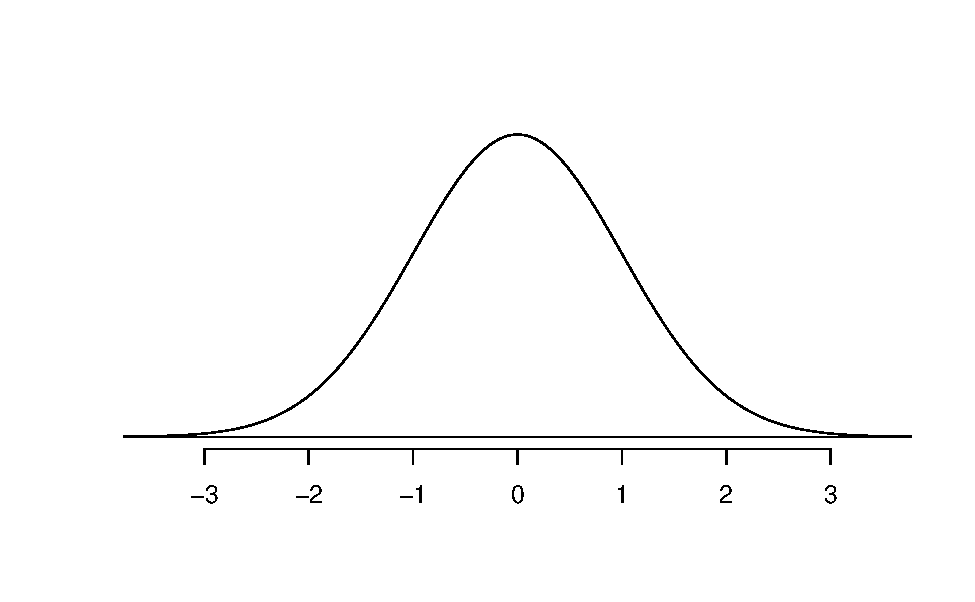
\includegraphics[width=0.6\linewidth]{09-A13-inference-2cat_test-theory_files/figure-latex/simpleNormal-1} 

}

\caption{A standard normal curve.}\label{fig:simpleNormal}
\end{figure}

\begin{enumerate}
\def\labelenumi{\arabic{enumi}.}
\setcounter{enumi}{7}
\tightlist
\item
  Mark the value of the standardized statistic on the standard normal distribution above and shade the area to find the p-value.
\end{enumerate}

\vspace{0.1in}

We will use the \texttt{pnorm()} function in R to find the p-value. Use the provided R script file and enter the value of the standardized statistic found in question 7 at \texttt{xx} in line 11; highlight and run lines 11--13.

\begin{Shaded}
\begin{Highlighting}[]
\FunctionTok{pnorm}\NormalTok{(xx, }\CommentTok{\# Enter value of standardized statistic}
      \AttributeTok{m=}\DecValTok{0}\NormalTok{, }\AttributeTok{s=}\DecValTok{1}\NormalTok{, }\CommentTok{\# Using the standard normal mean = 0, sd = 1}
      \AttributeTok{lower.tail=}\ConstantTok{TRUE}\NormalTok{) }\CommentTok{\# Gives a p{-}value less than the standardized statistic}
\end{Highlighting}
\end{Shaded}

\begin{enumerate}
\def\labelenumi{\arabic{enumi}.}
\setcounter{enumi}{8}
\item
  Report the p-value from the R output.
  \vspace{0.2in}
\item
  Interpret the p-value in context of the study.
\end{enumerate}

\vspace{1in}

\begin{enumerate}
\def\labelenumi{\arabic{enumi}.}
\setcounter{enumi}{10}
\tightlist
\item
  Write a conclusion to the research question based on the p-value found.
\end{enumerate}

\vspace{0.8in}

\begin{enumerate}
\def\labelenumi{\arabic{enumi}.}
\setcounter{enumi}{11}
\tightlist
\item
  Would a 90\% confidence interval contain the null value of zero? Explain your answer.
\end{enumerate}

\vspace{0.8in}
\newpage

\begin{enumerate}
\def\labelenumi{\arabic{enumi}.}
\setcounter{enumi}{12}
\tightlist
\item
  What is the scope of inference for this study?
\end{enumerate}

\vspace{0.8in}

\hypertarget{impacts-on-the-p-value}{%
\subsection*{Impacts on the p-value}\label{impacts-on-the-p-value}}
\addcontentsline{toc}{subsection}{Impacts on the p-value}

Suppose that we want to show that there is a \textbf{difference} in true proportion of head injuries for those that wear helmets and those that do not.

\begin{enumerate}
\def\labelenumi{\arabic{enumi}.}
\setcounter{enumi}{13}
\tightlist
\item
  Write out the alternative hypothesis in notation for this new research question.
\end{enumerate}

\vspace{0.3in}

\begin{enumerate}
\def\labelenumi{\arabic{enumi}.}
\setcounter{enumi}{14}
\tightlist
\item
  How would this impact the p-value?
\end{enumerate}

\vspace{0.2in}

Suppose in a larger sample of skiers and snowboarders involved in accidents we saw the following results.

\begin{longtable}[]{@{}cccc@{}}
\toprule()
& Helmet Use & No Helmet Use & Total \\
\midrule()
\endhead
Head Injury & 135 & 674 & 809 \\
No Head Injury & 921 & 3270 & 4191 \\
Total & 1056 & 3944 & 5000 \\
\bottomrule()
\end{longtable}

Note that the sample proportions for each group are the same as the smaller sample size.

\[\hat{p}_1 = \frac{135}{1056}=0.127, \hat{p}_2 = \frac{674}{3944}=0.171\]

\begin{enumerate}
\def\labelenumi{\arabic{enumi}.}
\setcounter{enumi}{15}
\tightlist
\item
  The standard error for the difference in proportions for this new sample is 0.013 (\(SE(\hat{p}_h - \hat{p}_n) = 0.013\)). Calculate the standardized statistic for this new sample.
\end{enumerate}

\vspace{0.8in}

Use Rstudio to find the p-value for this new sample. Enter the value of the standardized statistic found in question 16 for xx in line 18. Highlight and run lines 18--20.

\begin{Shaded}
\begin{Highlighting}[]
\FunctionTok{pnorm}\NormalTok{(xx, }\CommentTok{\# Enter value of standardized statistic}
      \AttributeTok{m=}\DecValTok{0}\NormalTok{, }\AttributeTok{s=}\DecValTok{1}\NormalTok{, }\CommentTok{\# Using the standard normal mean = 0, sd = 1}
      \AttributeTok{lower.tail=}\ConstantTok{TRUE}\NormalTok{) }\CommentTok{\# Gives a p{-}value greater than the standardized statistic}
\end{Highlighting}
\end{Shaded}

\newpage

\begin{enumerate}
\def\labelenumi{\arabic{enumi}.}
\setcounter{enumi}{16}
\tightlist
\item
  How does the increase in sample size affect the p-value?
\end{enumerate}

\vspace{0.4in}

\begin{enumerate}
\def\labelenumi{\arabic{enumi}.}
\setcounter{enumi}{17}
\tightlist
\item
  Suppose another sample of 3562 skiers and snowboarders was taken. In this new sample a difference in proportions of head injuries was found to be -0.009, (\(\hat{p}_h - \hat{p}_n = -0.009\)) with a standard error for the difference in proportions of 0.015, (\(SE(\hat{p}_h - \hat{p}_n) = 0.015\)). Calculate the standardized statistic for this new sample.
\end{enumerate}

\vspace{0.5in}

Use Rstudio to find the p-value for this new sample. Enter the value of the standardized statistic found in question 18 for xx in line 25. Highlight and run lines 25--27.

\begin{Shaded}
\begin{Highlighting}[]
\FunctionTok{pnorm}\NormalTok{(xx, }\CommentTok{\# Enter value of standardized statistic}
      \AttributeTok{m=}\DecValTok{0}\NormalTok{, }\AttributeTok{s=}\DecValTok{1} \CommentTok{\# Using the standard normal mean = 0, sd = 1}
      \AttributeTok{lower.tail=}\ConstantTok{TRUE}\NormalTok{) }\CommentTok{\# Gives a p{-}value greater than the standardized statistic}
\end{Highlighting}
\end{Shaded}

\begin{enumerate}
\def\labelenumi{\arabic{enumi}.}
\setcounter{enumi}{18}
\tightlist
\item
  How does a statistic closer to the null value affect the p-value?
\end{enumerate}

\vspace{0.3in}

\begin{enumerate}
\def\labelenumi{\arabic{enumi}.}
\setcounter{enumi}{19}
\tightlist
\item
  Summarize how each of the following affected the p-value:
\end{enumerate}

\begin{enumerate}
\def\labelenumi{\alph{enumi})}
\tightlist
\item
  Switching to a two-sided test.
\end{enumerate}

\vspace{0.4in}

\begin{enumerate}
\def\labelenumi{\alph{enumi})}
\setcounter{enumi}{1}
\tightlist
\item
  Using a larger sample size.
\end{enumerate}

\vspace{0.4in}

\begin{enumerate}
\def\labelenumi{\alph{enumi})}
\setcounter{enumi}{2}
\tightlist
\item
  Using a sample statistic closer to the null value.
\end{enumerate}

\vspace{0.4in}
\newpage

\hypertarget{take-home-messages}{%
\subsection{Take-home messages}\label{take-home-messages}}

\begin{enumerate}
\def\labelenumi{\arabic{enumi}.}
\item
  When comparing two groups, we are looking at the difference between two parameters. In the null hypothesis, we assume the two parameters are equal, or that there is no difference between the two proportions.
\item
  The standardized statistic when the response variable is categorical is a Z-score and is compared to the standard normal distribution to find the p-value. To find the standardized statistic, we take the value of the statistic minus the null value, divided by the null standard error of the statistic. The standardized statistic measures the number of standard errors the statistic is from the null value.
\item
  The p-value for a two-sided test is approximately two times the value for a one-sided test. A two-sided test provides less evidence against the null hypothesis.
\item
  The larger the sample size, the smaller the sample to sample variability. This will result in a larger standardized statistic and more evidence against the null hypothesis.
\item
  The farther the statistic is from the null value, the larger the standardized statistic. This will result in a smaller p-value and more evidence against the null hypothesis.
\end{enumerate}

\hypertarget{additional-notes}{%
\subsection{Additional notes}\label{additional-notes}}

Use this space to summarize your thoughts and take additional notes on today's activity and material covered.

\newpage

\hypertarget{activity-9b-winter-sports-helmet-use-and-head-injuries-theory-based-confidence-interval}{%
\section{Activity 9B: Winter Sports Helmet Use and Head Injuries --- Theory-based Confidence Interval}\label{activity-9b-winter-sports-helmet-use-and-head-injuries-theory-based-confidence-interval}}

\setstretch{1}

\hypertarget{learning-outcomes-1}{%
\subsection{Learning outcomes}\label{learning-outcomes-1}}

\begin{itemize}
\item
  Assess the conditions to use the normal distribution model for a difference in proportions.
\item
  Create and interpret a theory-based confidence interval for a difference in proportions.
\end{itemize}

\hypertarget{terminology-review-1}{%
\subsection{Terminology review}\label{terminology-review-1}}

In today's activity, we will use theory-based methods to estimate the difference in two proportions. Some terms covered in this activity are:

\begin{itemize}
\item
  Standard normal distribution
\item
  Independence and success-failure conditions
\end{itemize}

To review these concepts, see Chapter 15 in your textbook.

\hypertarget{winter-sports-helmet-use-and-head-injury}{%
\subsection{Winter sports helmet use and head injury}\label{winter-sports-helmet-use-and-head-injury}}

In this activity we will focus on theory-based methods to calculate a confidence interval. Recall from Activity 9A, the sampling distribution of a difference in proportions can be mathematically modeled using the normal distribution if certain conditions are met.

Conditions for the sampling distribution of \(\hat{p}_1-\hat{p}_2\) to follow an approximate normal distribution:

\begin{itemize}
\item
  \textbf{Independence}: The data are independent within and between the two groups. (\emph{Remember}: This also must be true to use simulation methods!)
\item
  \textbf{Success-failure condition}: This condition is met if we have at least 10 successes and 10 failures in each sample. Equivalently, we check that all cells in the table have at least 10 observations.
\end{itemize}

\begin{enumerate}
\def\labelenumi{\arabic{enumi}.}
\tightlist
\item
  Explain why a theory-based confidence interval for the data set in Activities 8A and 8B would NOT be similar to the bootstrap interval created.
\end{enumerate}

\vspace{1in}

For this activity we will again use the Helmet Use and Head Injury data set. In Activity 9A we saw that there was evidence that helmet use is associated with a reduced risk of head injury. Today we will estimate the difference in proportion of head injuries for those who wore helmets and those who did not.

In ``Helmet Use and Risk of Head Injuries in Alpine Skiers and Snowboarders'' by Sullheim et. al., (Sulheim et al. 2017), we can see the summary results from a random sample of 3562 skiers and snowboarders involved in accidents in the two-way table below.

\begin{longtable}[]{@{}cccc@{}}
\toprule()
& Helmet Use & No Helmet Use & Total \\
\midrule()
\endhead
Head Injury & 96 & 480 & 576 \\
No Head Injury & 656 & 2330 & 2986 \\
Total & 752 & 2810 & 3562 \\
\bottomrule()
\end{longtable}

\begin{enumerate}
\def\labelenumi{\arabic{enumi}.}
\setcounter{enumi}{1}
\tightlist
\item
  Write the parameter of interest for this study in context of the problem.
\end{enumerate}

\vspace{0.8in}

To find a confidence interval for the difference in proportions we will add and subtract the margin of error from the point estimate to find the two endpoints.

\[\hat{p}_1-\hat{p}_2\pm z^*\times SE(\hat{p}_1-\hat{p}_2), \hspace{.2cm} \text{where}\]
\[SE(\hat{p}_1-\hat{p}_2) = \sqrt{\frac{\hat{p}_1 (1-\hat{p}_1)}{n_1}+\frac{\hat{p}_2 (1-\hat{p}_2)}{n_2}}\]

Note that the formula changes when calculating the variability around the statistic in order to calculate a confidence interval from the formula used in Activity 9A! Here, we use the sample proportions for each group to calculate the standard error for the difference in proportions since we are not assuming that the true difference is zero.

To calculate the standard error for a difference in proportions to create a 90\% confidence interval we substitute in the two sample proportions and the sample size for each group into the equation above.

\[n_1 = 752, n_2 = 2810, \hat{p}_1 = \frac{96}{752} = 0.128, \hat{p}_2 = \frac{480}{2810} = 0.171\]

\[SE(\hat{p}_1-\hat{p}_2) = \sqrt{\frac{0.128 (1-0.128)}{752}+\frac{0.171 (1-0.171)}{2810}} = 0.014\]

Recall that the \(z^*\) multiplier is the percentile of a standard normal distribution that corresponds to our confidence level. If our confidence level is 90\%, we find the Z values that encompass the middle 90\% of the standard normal distribution. If 90\% of the standard normal distribution should be in the middle, that leaves 10\% in the tails, or 5\% in each tail. The \texttt{qnorm()} function in R will tell us the \(z^*\) value for the desired percentile (in this case, 90\% + 5\% = 95\% percentile).

\begin{Shaded}
\begin{Highlighting}[]
\FunctionTok{qnorm}\NormalTok{(}\FloatTok{0.95}\NormalTok{) }\CommentTok{\# Multiplier for 90\% confidence interval}
\end{Highlighting}
\end{Shaded}

\begin{verbatim}
#> [1] 1.644854
\end{verbatim}

\newpage

\begin{enumerate}
\def\labelenumi{\arabic{enumi}.}
\setcounter{enumi}{2}
\tightlist
\item
  Draw and label a standard normal distribution. Mark the value of the \(z^*\) multiplier adn the percentages used to find this muliplier.
\end{enumerate}

\vspace{1.5in}

Remember that the margin of error is the value added and subtracted to the sample difference in proportions to find the endpoints for the confidence interval.

\[ME = z^*\times SE(\hat{p}_1 - \hat{p}_2)\]

\begin{enumerate}
\def\labelenumi{\arabic{enumi}.}
\setcounter{enumi}{3}
\tightlist
\item
  Using the multiplier of \(z^*\) = 1.645 and the calculated standard error, calculate the margin of error for a 90\% confidence interval.
\end{enumerate}

\vspace{0.5in}

\begin{enumerate}
\def\labelenumi{\arabic{enumi}.}
\setcounter{enumi}{4}
\tightlist
\item
  Calculate the 90\% confidence interval for the parameter of interest.
\end{enumerate}

\vspace{0.8in}

\begin{enumerate}
\def\labelenumi{\arabic{enumi}.}
\setcounter{enumi}{5}
\tightlist
\item
  Interpret the confidence interval found in question 5 in context of the problem.
\end{enumerate}

\vspace{0.8in}

\begin{enumerate}
\def\labelenumi{\arabic{enumi}.}
\setcounter{enumi}{6}
\tightlist
\item
  Interpret the level of confidence in context of the problem. What does it mean to be 90\% confident in the confidence interval?
\end{enumerate}

\vspace{0.8in}

\begin{enumerate}
\def\labelenumi{\arabic{enumi}.}
\setcounter{enumi}{7}
\tightlist
\item
  What decision (reject or fail to reject the null hypothesis) would you make based on your confidence interval? Explain your answer.
  \vspace{0.5in}
  \newpage
\end{enumerate}

\hypertarget{effect-of-sample-size}{%
\subsection{Effect of sample size}\label{effect-of-sample-size}}

Suppose in another sample of skiers and snowboards involved in accidents we saw these results:

\begin{longtable}[]{@{}cccc@{}}
\toprule()
& Helmet Use & No Helmet Use & Total \\
\midrule()
\endhead
Head Injury & 135 & 674 & 809 \\
No Head Injury & 921 & 3270 & 4191 \\
Total & 1056 & 3944 & 5000 \\
\bottomrule()
\end{longtable}

Note that the sample proportions for each group are the same as the smaller sample size.

\[\hat{p}_1 = \frac{135}{1056}=0.127, \hat{p}_2 = \frac{674}{3944}=0.171\]

\begin{enumerate}
\def\labelenumi{\arabic{enumi}.}
\setcounter{enumi}{8}
\item
  Calculate the standard error for the difference in sample proportions for this new sample.
  \vspace{0.8in}
\item
  Calculate the margin of error for a 90\% confidence interval using a multiplier of \(z^*\) = 1.645 for this new sample. Is the margin of error larger or smaller than the margin of error for the original study?
  \vspace{.8in}
\item
  Calculate the 90\% confidence interval for this new study using the margin of error from question 10.\\
  \vspace{.8in}
\item
  Is the confidence interval calculated in question 11 with the larger sample size wider or narrower than the confidence interval in question 5? Why?
  \vspace{.8in}
\end{enumerate}

\newpage

\hypertarget{take-home-messages-1}{%
\subsection{Take-home messages}\label{take-home-messages-1}}

\begin{enumerate}
\def\labelenumi{\arabic{enumi}.}
\item
  Simulation-based methods and theory-based methods should give the same results for a study \emph{if the validity conditions are met}. For both methods, observational units need to be independent. To use theory-based methods, additionally, the success-failure condition must be met. Check the validity conditions for each type of test to determine if theory-based methods can be used.
\item
  When calculating the standard error for the difference in sample proportions when doing a hypothesis test, we use the pooled proportion of successes, the best estimate for calculating the variability \emph{under the assumption the null hypothesis is true}. For a confidence interval, we are not assuming a null hypothesis, so we use the values of the two conditional proportions to calculate the standard error. Make note of the difference in these two formulas.
\item
  Increasing sample size will result in less sample-to-sample variability in statistics, which will result in a smaller standard error, and thus a narrower confidence interval.
\end{enumerate}

\hypertarget{additional-notes-1}{%
\subsection{Additional notes}\label{additional-notes-1}}

Use this space to summarize your thoughts and take additional notes on today's activity and material covered.

\newpage

\hypertarget{week-9-lab-diabetes}{%
\section{Week 9 Lab: Diabetes}\label{week-9-lab-diabetes}}

\setstretch{1}

\hypertarget{learning-outcomes-2}{%
\subsection{Learning outcomes}\label{learning-outcomes-2}}

\begin{itemize}
\item
  Given a research question involving two categorical variables, construct the null and alternative hypotheses
  in words and using appropriate statistical symbols.
\item
  Assess the conditions to use the normal distribution model for a difference in proportions.
\item
  Describe and perform a simulation-based hypothesis test for a difference in proportions.
\item
  Calculate the Z test statistic for a difference in proportions.
\item
  Find, interpret, and evaluate the p-value for a hypothesis test for a difference in proportions.
\item
  Create and interpret a theory-based confidence interval for a difference in proportions.
\end{itemize}

\hypertarget{glycemic-control-in-diabetic-adolescents}{%
\subsection{Glycemic control in diabetic adolescents}\label{glycemic-control-in-diabetic-adolescents}}

Researchers compared the efficacy of two treatment regimens to achieve durable glycemic control in children and adolescents with recent-onset type 2 diabetes (Group 2012). A convenience sample of patients 10 to 17 years of age with recent-onset type 2 diabetes were randomly assigned to either a medication (rosiglitazone) or a lifestyle-intervention program focusing on weight loss through eating and activity. Researchers measured whether the patient still needs insulin (failure) or had glycemic control (success). Of the 233 children who received the Rosiglitazone treatment, 143 had glycemic control, while of the 234 who went through the lifestyle-intervention program, 125 had glycemic control. Is there evidence that there is difference in proportion of patients that achieve durable glycemic control between the two treatments? Use Rosiglitazone -- Lifestyle as the order of subtraction.

Upload and open the R script file for Week 9 lab. Upload and import the csv file, \texttt{diabetes}. Enter the name of the data set (see the environment tab) for \texttt{datasetname} in the R script file in line 7. Highlight and run lines 1--8 to get the counts for each combination of categories.

\begin{Shaded}
\begin{Highlighting}[]
\NormalTok{glycemic }\OtherTok{\textless{}{-}}\NormalTok{ datasetname}
\NormalTok{glycemic }\SpecialCharTok{\%\textgreater{}\%} \FunctionTok{group\_by}\NormalTok{(treatment) }\SpecialCharTok{\%\textgreater{}\%} \FunctionTok{count}\NormalTok{(outcome)}
\end{Highlighting}
\end{Shaded}

\begin{enumerate}
\def\labelenumi{\arabic{enumi}.}
\item
  Is this an experiment or an observational study?
  \vspace{0.2in}
\item
  Complete the following two-way table using the R output.
\end{enumerate}

\begin{center}
\begin{tabular}{|c|c|c|c|}\hline
 & \multicolumn{2}{|c|}{\textbf{Treatment}} & \\ \hline
\textbf{Outcome} & Rosiglitazone & Lifestyle & Total \\ \hline
 Glycemic Control & & & \\ 
 & & & \\ \hline
 Insulin Required & & & \\ 
 & & & \\ \hline
 Total & & &  \\ 
 & & & \\ \hline  
\end{tabular}
\end{center}

\begin{enumerate}
\def\labelenumi{\arabic{enumi}.}
\setcounter{enumi}{2}
\item
  Is the independence condition met for this study? Explain your answer.
  \vspace{0.6in}
\item
  Write the parameter of interest for the research question.
  \vspace{0.6in}
\item
  Using the research question, write the alternative hypothesis in notation.
  \vspace{0.3in}
\item
  \textbf{Calculate the summary statistic (difference in proportions). Use appropriate notation.}
  \vspace{0.3in}
\end{enumerate}

Fill in the missing values/names in the R script file in the two-proportion\_test function to create the null distribution and find the simulation p-value for the test.

\begin{Shaded}
\begin{Highlighting}[]
\FunctionTok{two\_proportion\_test}\NormalTok{(}\AttributeTok{formula =}\NormalTok{ outcome}\SpecialCharTok{\textasciitilde{}}\NormalTok{treatment, }\CommentTok{\# response \textasciitilde{} explanatory}
         \AttributeTok{data=}\NormalTok{ glycemic, }\CommentTok{\# Name of data set}
         \AttributeTok{first\_in\_subtraction =} \StringTok{"xx"}\NormalTok{, }\CommentTok{\# Order of subtraction: enter the name of Group 1}
         \AttributeTok{number\_repetitions =} \DecValTok{1000}\NormalTok{, }\CommentTok{\# Always use a minimum of 1000 repetitions}
         \AttributeTok{response\_value\_numerator =} \StringTok{"xx"}\NormalTok{, }\CommentTok{\# Define which outcome is a success }
         \AttributeTok{as\_extreme\_as =}\NormalTok{ xx, }\CommentTok{\# Calculated observed statistic (difference in sample proportions)}
         \AttributeTok{direction=}\StringTok{"xx"}\NormalTok{) }\CommentTok{\# Alternative hypothesis direction ("greater","less","two{-}sided")}
\end{Highlighting}
\end{Shaded}

\begin{enumerate}
\def\labelenumi{\arabic{enumi}.}
\setcounter{enumi}{6}
\item
  Report the p-value. How much evidence does the p-value provide against the null hypothesis?
  \vspace{0.3in}
\item
  \textbf{Will the theory-based p-value be similar to the simulation p-value? Explain your answer.}
  \vspace{0.8in}
\item
  \textbf{Calculate the number of standard errors the sample difference in proportion is from the null value of zero.}
  \vspace{0.8in}
\item
  \textbf{Will a 95\% simulation confidence interval contain the null value of zero? Explain your answer.}
  \vspace{0.8in}
\item
  Calculate the standard error for a difference in proportions to create a 95\% confidence interval.\\
  \vspace{1in}
\item
  Use the multiplier of \(z^*\) = 1.96 and the standard error found in question 11 to calculate a 95\% confidence interval for the parameter of interest.
  \vspace{1in}
\item
  Write a paragraph summarizing the results of the study. Be sure to describe:
\end{enumerate}

\begin{itemize}
\item
  Summary statistic and interpretation
\item
  P-value and interpretation

  \begin{itemize}
  \item
    Statement about probability or proportion of samples
  \item
    Statistic (summary measure and value)
  \item
    Direction of the alternative
  \item
    Null hypothesis (in context)
  \end{itemize}
\item
  Confidence interval and interpretation

  \begin{itemize}
  \item
    How confident you are (e.g., 90\%, 95\%, 98\%, 99\%)
  \item
    Parameter of interest
  \item
    Calculated interval
  \item
    Order of subtraction when comparing two groups
  \end{itemize}
\item
  Conclusion (written to answer the research question)

  \begin{itemize}
  \item
    Amount of evidence
  \item
    Parameter of interest
  \item
    Direction of the alternative hypothesis
  \end{itemize}
\item
  Scope of inference

  \begin{itemize}
  \item
    To what group of observational units do the results apply (target population or observational units similar to the sample)?
  \item
    What type of inference is appropriate (causal or non-causal)?
  \end{itemize}
\end{itemize}

\textbf{Upload a copy of your group's p-value interpretation and scope of inference to Gradescope.}

\newpage

Paragraph (continued):

\newpage

\hypertarget{group-exam-2-review}{%
\chapter{Group Exam 2 Review}\label{group-exam-2-review}}

Use the provided data set from the Islands (ExamReviewData.csv) and the appropriate Exam 1 Review R script file to answer the following questions. Each adult (\textgreater21) islander was selected at random from all adult islanders. Note that some islanders choose not to participate in the study. These islanders that did not consent to be in the study are removed from the dataset before analysis. Variables and their descriptions are listed below.

\begin{longtable}[]{@{}
  >{\raggedright\arraybackslash}p{(\columnwidth - 2\tabcolsep) * \real{0.2353}}
  >{\raggedright\arraybackslash}p{(\columnwidth - 2\tabcolsep) * \real{0.7647}}@{}}
\toprule()
\begin{minipage}[b]{\linewidth}\raggedright
\textbf{Variable}
\end{minipage} & \begin{minipage}[b]{\linewidth}\raggedright
\textbf{Description}
\end{minipage} \\
\midrule()
\endhead
\texttt{Island} & Name of Island that the Islander resides on \\
\texttt{City} & Name of City in which the Islander resides \\
\texttt{Population} & Population of the City \\
\texttt{Name} & Name of Islander \\
\texttt{Consent} & Whether the Islander consented to be in the study \\
\texttt{Gender} & Gender of Islander (M = male, F = Female) \\
\texttt{Age} & Age of Islander \\
\texttt{Married} & Marital status of Islander \\
\texttt{Smoking\_Status} & Whether the Islander is a current smoker \\
\texttt{Children} & Whether the Islander has children \\
\texttt{weight\_kg} & Weight measured in kg \\
\texttt{height\_cm} & Height measured in cm \\
\texttt{respiratory\_rate} & Breaths per minute \\
\texttt{Type\_of\_Music} & Music type (Classical or Heavy Medal) Islander was randomly assigned to listen to \\
\texttt{After\_PuzzleCube} & Time to complete puzzle cube (minutes) after listening to assigned music \\
\texttt{Education\_Level} & Highest level of education completed \\
\texttt{Balance\_Test} & Time balanced measured in seconds with eyes closed \\
\texttt{Blood\_Glucose\_before} & Level of blood glucose (mg/dL) before consuming assigned drink \\
\texttt{Heart\_Rate\_before} & Heart rate (bpm) before consuming assigned drink \\
\texttt{Blood\_Glucose\_after} & Level of blood glucose (mg/dL) after consuming assigned drink \\
\texttt{Heart\_Rate\_after} & Heart rate (bpm) after consuming assigned drink \\
\texttt{Diff\_Heart\_Rate} & Difference in heart rate (bpm) for Before - After consuming assigned drink \\
\texttt{Diff\_Blood\_Glucose} & Difference in blood glucose (mg/dL) for Before - After consuming assigned drink \\
\bottomrule()
\end{longtable}

\newpage

\begin{enumerate}
\def\labelenumi{\arabic{enumi}.}
\tightlist
\item
  Use the appropriate Exam 2 Review R script file and analyze the following research question: ``Is there evidence that those with a higher education level are less likely to smoke?''
\end{enumerate}

\begin{enumerate}
\def\labelenumi{\alph{enumi}.}
\item
  Parameter of Interest:
  \vspace{0.3in}
\item
  Null Hypothesis:

  Notation:
  \vspace{0.3in}

  Words:
  \vspace{0.5in}
\item
  Alternative Hypothesis:

  Notation:
  \vspace{0.3in}

  Words:
  \vspace{0.5in}
\item
  Use the R script file to get the counts for each level and combination of variables. Fill in the following table with the variable names, levels of each variable, and counts using the values from the R output.
\end{enumerate}

\begingroup
\setlength{\tabcolsep}{14pt}
\renewcommand{\arraystretch}{2}
\begin{center}
\begin{tabular}{|c|p{1in}|p{1in}|p{1in}|}
\hline
 & \multicolumn{2}{|c|}{\textbf{Explanatory Variable}} & \\ 
 & \multicolumn{2}{|c|}{ } & \\ \hline
\textbf{Response variable} & Group 1 & Group 2 & Total \\
 & & & \\ \hline
 Success & & & \\
 & & & \\ \hline
 Failure & & & \\
 & & & \\ \hline
 Total & & & \\
 & & & \\ \hline
\end{tabular}
\end{center}
\endgroup

\begin{enumerate}
\def\labelenumi{\alph{enumi}.}
\setcounter{enumi}{4}
\tightlist
\item
  Calculate the value of the summary statistic to answer the research question. Give appropriate notation.
\end{enumerate}

\vspace{0.4in}

\begin{enumerate}
\def\labelenumi{\alph{enumi}.}
\setcounter{enumi}{5}
\tightlist
\item
  Interpret the value of the summary statistic in context of the problem:
\end{enumerate}

\vspace{0.4in}

\begin{enumerate}
\def\labelenumi{\alph{enumi}.}
\setcounter{enumi}{6}
\item
  Assess if the following conditions are met:

  Independence (needed for both simulation and theory-based methods):
  \vspace{0.8in}

  Success-Failure (must be met to use theory-based methods):
  \vspace{0.8in}
\item
  Use the provided R script file to find the simulation p-value to assess the research question. Report the p-value.
  \vspace{0.3in}
\item
  Interpret the p-value in the context of the problem.
  \vspace{0.8in}
\item
  Write a conclusion to the research question based on the p-value.
  \vspace{0.8in}
\item
  Using a significance level of \(\alpha = 0.05\), what statistical decision will you make about the null hypothesis?
  \vspace{0.3in}
\item
  Use the provided R script file to find a 95\% confidence interval.
  \vspace{0.3in}
\item
  Interpret the 95\% confidence interval in context of the problem.
  \vspace{0.8in}
\item
  Regardless to your answer in part g, calculate the standardized statistic.
  \vspace{0.4in}
\item
  Interpret the value of the standardized statistic in context of the problem.
  \vspace{0.8in}
\item
  Use the provided R script file to find the theory-based p-value.
  \vspace{0.3in}
\item
  Use the provided R script file to find the appropriate z* multiplier and calculate the theory-based confidence interval.
  \vspace{0.5in}
\item
  Does the theory-based p-value and CI match those found using simulation methods? Explain why or why not.
  \vspace{0.8in}
\item
  What is the scope of inference for this study?
  \vspace{0.8in}
\end{enumerate}

\newpage

\hypertarget{refs}{}
\begin{CSLReferences}{1}{0}
\leavevmode\vadjust pre{\hypertarget{ref-pga}{}}%
{``Average Driving Distance and Fairway Accuracy.''} 2008. \href{https://www.pga.com/\%20and\%20https://www.lpga.com/}{https://www.pga.com/ and https://www.lpga.com/}.

\leavevmode\vadjust pre{\hypertarget{ref-islands}{}}%
Bulmer, M. n.d. {``Islands in Schools Project.''} \url{https://sites.google.com/site/islandsinschoolsprojectwebsite/home}.

\leavevmode\vadjust pre{\hypertarget{ref-darley1973}{}}%
Darley, J. M., and C. D. Batson. 1973. {``"From Jerusalem to Jericho": A Study of Situational and Dispositional Variables in Helping Behavior.''} \emph{Journal of Personality and Social Psychology} 27: 100--108.

\leavevmode\vadjust pre{\hypertarget{ref-ipeds}{}}%
Education Statistics, National Center for. 2018. {``IPEDS.''} \url{https://nces.ed.gov/ipeds/}.

\leavevmode\vadjust pre{\hypertarget{ref-zeitler2012}{}}%
Group, TODAY Study. 2012. {``\href{https://www.ncbi.nlm.nih.gov/pubmed/22540912}{A Clinical Trial to Maintain Glycemic Control in Youth with Type 2 Diabetes}.''} \emph{New England Journal of Medicine} 366: 2247--56.

\leavevmode\vadjust pre{\hypertarget{ref-hamblin2007}{}}%
Hamblin, J. K., K. Wynn, and P. Bloom. 2007. {``Social Evaluation by Preverbal Infants.''} \emph{Nature} 450 (6288): 557--59.

\leavevmode\vadjust pre{\hypertarget{ref-hirschfelder2018}{}}%
Hirschfelder, A., and P. F. Molin. 2018. {``I Is for Ignoble: Stereotyping Native Americans.''} \href{Retrieved\%20from\%20https://www.ferris.edu/HTMLS/news/jimcrow/native/homepage.htm.}{Retrieved from https://www.ferris.edu/HTMLS/news/jimcrow/native/homepage.htm.}

\leavevmode\vadjust pre{\hypertarget{ref-imdb}{}}%
{``{IMDb} Movies Extensive Dataset.''} 2016. \url{https://kaggle.com/stefanoleone992/imdb-extensive-dataset}.

\leavevmode\vadjust pre{\hypertarget{ref-keating2021}{}}%
Keating, D., N. Ahmed, F. Nirappil, Stanley-Becker I., and L. Bernstein. 2021. {``Coronavirus Infections Dropping Where People Are Vaccinated, Rising Where They Are Not, Post Analysis Finds.''} \emph{Washington Post}. \url{https://www.washingtonpost.com/health/2021/06/14/covid-cases-vaccination-rates/}.

\leavevmode\vadjust pre{\hypertarget{ref-becentispeech}{}}%
Moquin, W., and C. Van Doren. 1973. {``Great Documents in American Indian History.''} Praeger.

\leavevmode\vadjust pre{\hypertarget{ref-obrien2019}{}}%
O'Brien, Lynch, H. D. 2019. {``Crocodylian Head Width Allometry and Phylogenetic Prediction of Body Size in Extinct Crocodyliforms.''} \emph{Integrative Organismal Biology} 1.

\leavevmode\vadjust pre{\hypertarget{ref-porath2017}{}}%
Porath, Erez, C. 2017. {``Does Rudeness Really Matter? The Effects of Rudeness on Task Performance and Helpfulness.''} \emph{Academy of Management Journal} 50.

\leavevmode\vadjust pre{\hypertarget{ref-quinn1999}{}}%
Quinn, G. E., C. H. Shin, M. G. Maguire, and R. A. Stone. 1999. {``Myopia and Ambient Lighting at Night.''} \emph{Nature} 399 (6732): 113--14. \url{https://doi.org/10.1038/20094}.

\leavevmode\vadjust pre{\hypertarget{ref-cdchospitalization}{}}%
{``Rates of Laboratory-Confimed COVID-19 Hospitalizations by Vaccination Status.''} 2021. CDC. \url{https://covid.cdc.gov/covid-data-tracker/\#covidnet-hospitalizations-vaccination}.

\leavevmode\vadjust pre{\hypertarget{ref-richardson2019}{}}%
Richardson, T., and R. T. Gilman. 2019. {``Left-Handedness Is Associated with Greater Fighting Success in Humans.''} \emph{Scientific Reports} 9 (1): 15402. \url{https://doi.org/10.1038/s41598-019-51975-3}.

\leavevmode\vadjust pre{\hypertarget{ref-stephens2020}{}}%
Stephens, R., and O. Robertson. 2020. {``Swearing as a Response to Pain: Assessing Hypoalgesic Effects of Novel "Swear" Words.''} \emph{Frontiers in Psychology} 11: 643--62.

\leavevmode\vadjust pre{\hypertarget{ref-stewart2014}{}}%
Stewart, E. H., B. Davis, B. L. Clemans-Taylor, B. Littenberg, C. A. Estrada, and R. M. Centor. 2014. {``Rapid Antigen Group a Streptococcus Test to Diagnose Pharyngitis: A Systematic Review and Meta-Analysis''} 9 (11). \url{https://doi.org/10.1371/journal.pone.0111727}.

\leavevmode\vadjust pre{\hypertarget{ref-stroop1935}{}}%
Stroop, J. R. 1935. {``Studies of Interference in Serial Verbal Reactions.''} \emph{Journal of Experimental Psychology} 18: 643--62.

\leavevmode\vadjust pre{\hypertarget{ref-sulheim2017}{}}%
Sulheim, S., A. Ekeland, I. Holme, and R. Bahr. 2017. {``Helmet Use and Risk of Head Injuries in Alpine Skiers and Snowboarders: Changes After an Interval of One Decade''} 51 (1): 44--50. \url{https://doi.org/10.1136/bjsports-2015-095798}.

\leavevmode\vadjust pre{\hypertarget{ref-titanic}{}}%
{``Titanic.''} n.d. \url{http://www.encyclopedia-titanica.org}.

\leavevmode\vadjust pre{\hypertarget{ref-covidvaccinetracker}{}}%
{``US COVID-19 Vaccine Tracker: See Your State's Progress.''} 2021. Mayo Clinic. \url{https://www.mayoclinic.org/coronavirus-covid-19/vaccine-tracker}.

\leavevmode\vadjust pre{\hypertarget{ref-navajo2011}{}}%
{``Welcome to the Navajo Nation Government: Official Site of the Navajo Nation.''} 2011.\href{\%20Retrieved\%20from\%20https://www.navajo-nsn.gov/.}{Retrieved from https://www.navajo-nsn.gov/.}

\leavevmode\vadjust pre{\hypertarget{ref-wilson2016}{}}%
Wilson, Woodruff, J. P. 2016. {``Vertebral Adaptations to Large Body Size in Theropod Dinosaurs.''} \emph{PLoS ONE} 11(7).

\end{CSLReferences}

\end{document}
